\documentclass[11pt,a4paper]{amsart}

\title{$C_6$.}

\usepackage[a4paper,margin=1in]{geometry}
\usepackage[euler-digits]{eulervm}
\usepackage{tikz}
\usetikzlibrary{calc}

\begin{document}
%\maketitle
\section*{$C_6$.}

\begin{align*}
  \left(
  \begin{array}{c|c|c|c}
    1&2&3&4\\
\hline
    5&6&7&8\\
\hline
    9&10&11&12\\
\hline
    13&14&15&16\\
  \end{array}
\right)
  \left(
  \begin{array}{c|c}
    17&18\\
\hline
    19&20\\
  \end{array}
\right)
  \left(
  \begin{array}{cc|cc}
    21&22&23&24\\
    22&21&24&23\\
\hline
    25&26&27&28\\
    26&25&28&27\\
  \end{array}
\right)
  \left(
  \begin{array}{cc}
    29&30\\
    30&29\\
  \end{array}
\right)
\end{align*}

\tikzset{every picture/.style={scale=0.20,nodes={rectangle,fill=black!50!green,inner sep=1mm}}}
% gap> for r in reps do
% > Print(TikzRelationSubgroup(GG, elm, r));
% > Print("\\quad\n");
% > od;
% \begin{center}
% \begin{tikzpicture}
% \draw (0,5) node {};
% \draw[shift={(-0.5,-0.5)},black!30,very thin](0,0) grid (6,6);
% \end{tikzpicture}
% \quad
% \begin{tikzpicture}
% \draw (0,5) node {};
% \draw (3,5) node {};
% \draw[shift={(-0.5,-0.5)},black!30,very thin](0,0) grid (6,6);
% \end{tikzpicture}
% \quad
% \begin{tikzpicture}
% \draw (0,5) node {};
% \draw (2,5) node {};
% \draw (4,5) node {};
% \draw[shift={(-0.5,-0.5)},black!30,very thin](0,0) grid (6,6);
% \end{tikzpicture}
% \quad
% \begin{tikzpicture}
% \draw (0,5) node {};
% \draw (1,5) node {};
% \draw (2,5) node {};
% \draw (3,5) node {};
% \draw (4,5) node {};
% \draw (5,5) node {};
% \draw[shift={(-0.5,-0.5)},black!30,very thin](0,0) grid (6,6);
% \end{tikzpicture}
% \quad
% \begin{tikzpicture}
% \draw (0,5) node {};
% \draw (0,2) node {};
% \draw[shift={(-0.5,-0.5)},black!30,very thin](0,0) grid (6,6);
% \end{tikzpicture}
% \quad
% \begin{tikzpicture}
% \draw (0,5) node {};
% \draw (3,5) node {};
% \draw (0,2) node {};
% \draw (3,2) node {};
% \draw[shift={(-0.5,-0.5)},black!30,very thin](0,0) grid (6,6);
% \end{tikzpicture}
% \quad
% \begin{tikzpicture}
% \draw (0,5) node {};
% \draw (2,5) node {};
% \draw (4,5) node {};
% \draw (0,2) node {};
% \draw (2,2) node {};
% \draw (4,2) node {};
% \draw[shift={(-0.5,-0.5)},black!30,very thin](0,0) grid (6,6);
% \end{tikzpicture}
% \quad
% \begin{tikzpicture}
% \draw (0,5) node {};
% \draw (1,5) node {};
% \draw (2,5) node {};
% \draw (3,5) node {};
% \draw (4,5) node {};
% \draw (5,5) node {};
% \draw (0,2) node {};
% \draw (1,2) node {};
% \draw (2,2) node {};
% \draw (3,2) node {};
% \draw (4,2) node {};
% \draw (5,2) node {};
% \draw[shift={(-0.5,-0.5)},black!30,very thin](0,0) grid (6,6);
% \end{tikzpicture}
% \quad
% \begin{tikzpicture}
% \draw (0,5) node {};
% \draw (0,3) node {};
% \draw (0,1) node {};
% \draw[shift={(-0.5,-0.5)},black!30,very thin](0,0) grid (6,6);
% \end{tikzpicture}
% \quad
% \begin{tikzpicture}
% \draw (0,5) node {};
% \draw (3,5) node {};
% \draw (0,3) node {};
% \draw (3,3) node {};
% \draw (0,1) node {};
% \draw (3,1) node {};
% \draw[shift={(-0.5,-0.5)},black!30,very thin](0,0) grid (6,6);
% \end{tikzpicture}
% \quad
% \begin{tikzpicture}
% \draw (0,5) node {};
% \draw (2,5) node {};
% \draw (4,5) node {};
% \draw (0,3) node {};
% \draw (2,3) node {};
% \draw (4,3) node {};
% \draw (0,1) node {};
% \draw (2,1) node {};
% \draw (4,1) node {};
% \draw[shift={(-0.5,-0.5)},black!30,very thin](0,0) grid (6,6);
% \end{tikzpicture}
% \quad
% \begin{tikzpicture}
% \draw (0,5) node {};
% \draw (1,5) node {};
% \draw (2,5) node {};
% \draw (3,5) node {};
% \draw (4,5) node {};
% \draw (5,5) node {};
% \draw (0,3) node {};
% \draw (1,3) node {};
% \draw (2,3) node {};
% \draw (3,3) node {};
% \draw (4,3) node {};
% \draw (5,3) node {};
% \draw (0,1) node {};
% \draw (1,1) node {};
% \draw (2,1) node {};
% \draw (3,1) node {};
% \draw (4,1) node {};
% \draw (5,1) node {};
% \draw[shift={(-0.5,-0.5)},black!30,very thin](0,0) grid (6,6);
% \end{tikzpicture}
% \quad
% \begin{tikzpicture}
% \draw (0,5) node {};
% \draw (0,4) node {};
% \draw (0,3) node {};
% \draw (0,2) node {};
% \draw (0,1) node {};
% \draw (0,0) node {};
% \draw[shift={(-0.5,-0.5)},black!30,very thin](0,0) grid (6,6);
% \end{tikzpicture}
% \quad
% \begin{tikzpicture}
% \draw (0,5) node {};
% \draw (3,5) node {};
% \draw (0,4) node {};
% \draw (3,4) node {};
% \draw (0,3) node {};
% \draw (3,3) node {};
% \draw (0,2) node {};
% \draw (3,2) node {};
% \draw (0,1) node {};
% \draw (3,1) node {};
% \draw (0,0) node {};
% \draw (3,0) node {};
% \draw[shift={(-0.5,-0.5)},black!30,very thin](0,0) grid (6,6);
% \end{tikzpicture}
% \quad
% \begin{tikzpicture}
% \draw (0,5) node {};
% \draw (2,5) node {};
% \draw (4,5) node {};
% \draw (0,4) node {};
% \draw (2,4) node {};
% \draw (4,4) node {};
% \draw (0,3) node {};
% \draw (2,3) node {};
% \draw (4,3) node {};
% \draw (0,2) node {};
% \draw (2,2) node {};
% \draw (4,2) node {};
% \draw (0,1) node {};
% \draw (2,1) node {};
% \draw (4,1) node {};
% \draw (0,0) node {};
% \draw (2,0) node {};
% \draw (4,0) node {};
% \draw[shift={(-0.5,-0.5)},black!30,very thin](0,0) grid (6,6);
% \end{tikzpicture}
% \quad
% \begin{tikzpicture}
% \draw (0,5) node {};
% \draw (1,5) node {};
% \draw (2,5) node {};
% \draw (3,5) node {};
% \draw (4,5) node {};
% \draw (5,5) node {};
% \draw (0,4) node {};
% \draw (1,4) node {};
% \draw (2,4) node {};
% \draw (3,4) node {};
% \draw (4,4) node {};
% \draw (5,4) node {};
% \draw (0,3) node {};
% \draw (1,3) node {};
% \draw (2,3) node {};
% \draw (3,3) node {};
% \draw (4,3) node {};
% \draw (5,3) node {};
% \draw (0,2) node {};
% \draw (1,2) node {};
% \draw (2,2) node {};
% \draw (3,2) node {};
% \draw (4,2) node {};
% \draw (5,2) node {};
% \draw (0,1) node {};
% \draw (1,1) node {};
% \draw (2,1) node {};
% \draw (3,1) node {};
% \draw (4,1) node {};
% \draw (5,1) node {};
% \draw (0,0) node {};
% \draw (1,0) node {};
% \draw (2,0) node {};
% \draw (3,0) node {};
% \draw (4,0) node {};
% \draw (5,0) node {};
% \draw[shift={(-0.5,-0.5)},black!30,very thin](0,0) grid (6,6);
% \end{tikzpicture}
% \quad
% \begin{tikzpicture}
% \draw (0,5) node {};
% \draw (3,2) node {};
% \draw[shift={(-0.5,-0.5)},black!30,very thin](0,0) grid (6,6);
% \end{tikzpicture}
% \quad
% \begin{tikzpicture}
% \draw (0,5) node {};
% \draw (2,5) node {};
% \draw (4,5) node {};
% \draw (1,2) node {};
% \draw (3,2) node {};
% \draw (5,2) node {};
% \draw[shift={(-0.5,-0.5)},black!30,very thin](0,0) grid (6,6);
% \end{tikzpicture}
% \quad
% \begin{tikzpicture}
% \draw (0,5) node {};
% \draw (3,4) node {};
% \draw (0,3) node {};
% \draw (3,2) node {};
% \draw (0,1) node {};
% \draw (3,0) node {};
% \draw[shift={(-0.5,-0.5)},black!30,very thin](0,0) grid (6,6);
% \end{tikzpicture}
% \quad
% \begin{tikzpicture}
% \draw (0,5) node {};
% \draw (2,5) node {};
% \draw (4,5) node {};
% \draw (1,4) node {};
% \draw (3,4) node {};
% \draw (5,4) node {};
% \draw (0,3) node {};
% \draw (2,3) node {};
% \draw (4,3) node {};
% \draw (1,2) node {};
% \draw (3,2) node {};
% \draw (5,2) node {};
% \draw (0,1) node {};
% \draw (2,1) node {};
% \draw (4,1) node {};
% \draw (1,0) node {};
% \draw (3,0) node {};
% \draw (5,0) node {};
% \draw[shift={(-0.5,-0.5)},black!30,very thin](0,0) grid (6,6);
% \end{tikzpicture}
% \quad
% \begin{tikzpicture}
% \draw (0,5) node {};
% \draw (2,3) node {};
% \draw (4,1) node {};
% \draw[shift={(-0.5,-0.5)},black!30,very thin](0,0) grid (6,6);
% \end{tikzpicture}
% \quad
% \begin{tikzpicture}
% \draw (0,5) node {};
% \draw (4,3) node {};
% \draw (2,1) node {};
% \draw[shift={(-0.5,-0.5)},black!30,very thin](0,0) grid (6,6);
% \end{tikzpicture}
% \quad
% \begin{tikzpicture}
% \draw (0,5) node {};
% \draw (3,5) node {};
% \draw (2,3) node {};
% \draw (5,3) node {};
% \draw (1,1) node {};
% \draw (4,1) node {};
% \draw[shift={(-0.5,-0.5)},black!30,very thin](0,0) grid (6,6);
% \end{tikzpicture}
% \quad
% \begin{tikzpicture}
% \draw (0,5) node {};
% \draw (3,5) node {};
% \draw (1,3) node {};
% \draw (4,3) node {};
% \draw (2,1) node {};
% \draw (5,1) node {};
% \draw[shift={(-0.5,-0.5)},black!30,very thin](0,0) grid (6,6);
% \end{tikzpicture}
% \quad
% \begin{tikzpicture}
% \draw (0,5) node {};
% \draw (4,4) node {};
% \draw (2,3) node {};
% \draw (0,2) node {};
% \draw (4,1) node {};
% \draw (2,0) node {};
% \draw[shift={(-0.5,-0.5)},black!30,very thin](0,0) grid (6,6);
% \end{tikzpicture}
% \quad
% \begin{tikzpicture}
% \draw (0,5) node {};
% \draw (2,4) node {};
% \draw (4,3) node {};
% \draw (0,2) node {};
% \draw (2,1) node {};
% \draw (4,0) node {};
% \draw[shift={(-0.5,-0.5)},black!30,very thin](0,0) grid (6,6);
% \end{tikzpicture}
% \quad
% \begin{tikzpicture}
% \draw (0,5) node {};
% \draw (3,5) node {};
% \draw (1,4) node {};
% \draw (4,4) node {};
% \draw (2,3) node {};
% \draw (5,3) node {};
% \draw (0,2) node {};
% \draw (3,2) node {};
% \draw (1,1) node {};
% \draw (4,1) node {};
% \draw (2,0) node {};
% \draw (5,0) node {};
% \draw[shift={(-0.5,-0.5)},black!30,very thin](0,0) grid (6,6);
% \end{tikzpicture}
% \quad
% \begin{tikzpicture}
% \draw (0,5) node {};
% \draw (3,5) node {};
% \draw (2,4) node {};
% \draw (5,4) node {};
% \draw (1,3) node {};
% \draw (4,3) node {};
% \draw (0,2) node {};
% \draw (3,2) node {};
% \draw (2,1) node {};
% \draw (5,1) node {};
% \draw (1,0) node {};
% \draw (4,0) node {};
% \draw[shift={(-0.5,-0.5)},black!30,very thin](0,0) grid (6,6);
% \end{tikzpicture}
% \quad
% \begin{tikzpicture}
% \draw (0,5) node {};
% \draw (1,4) node {};
% \draw (2,3) node {};
% \draw (3,2) node {};
% \draw (4,1) node {};
% \draw (5,0) node {};
% \draw[shift={(-0.5,-0.5)},black!30,very thin](0,0) grid (6,6);
% \end{tikzpicture}
% \quad
% \begin{tikzpicture}
% \draw (0,5) node {};
% \draw (5,4) node {};
% \draw (4,3) node {};
% \draw (3,2) node {};
% \draw (2,1) node {};
% \draw (1,0) node {};
% \draw[shift={(-0.5,-0.5)},black!30,very thin](0,0) grid (6,6);
% \end{tikzpicture}
% \quad
% % gap> LogTo();
% \end{center}
%
\tiny
\arraycolsep2pt
\begin{align*}
%   gap> for i in [1..30] do
% > Print(LaTeX(mmm[i]/(diam[i][i]/6)));
% > Print("\\quad\n");
% > od;
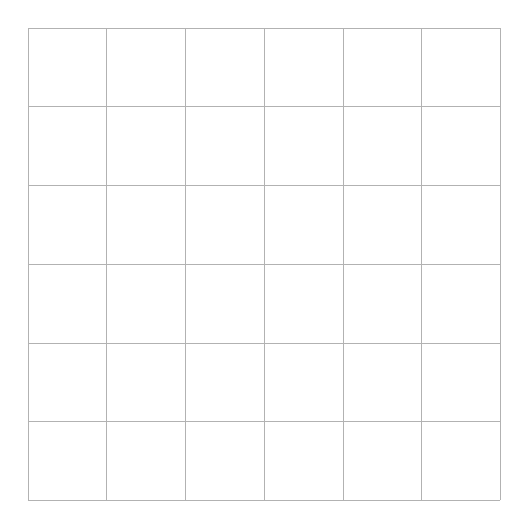
\begin{tikzpicture}
\draw (0,5) node {};
\draw[shift={(-0.5,-0.5)},black!30,very thin](0,0) grid (6,6);
\end{tikzpicture}
\quad
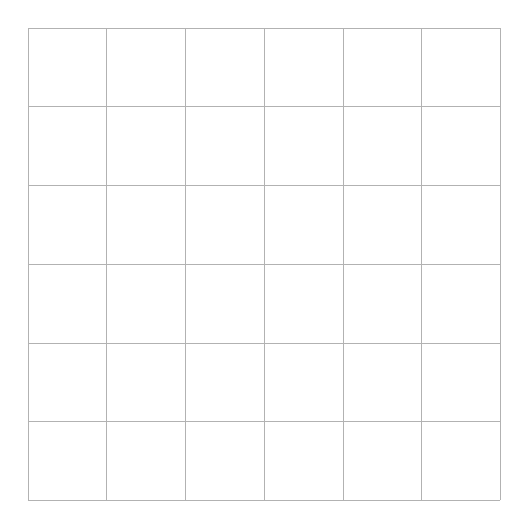
\begin{tikzpicture}
\draw (0,5) node {};
\draw (1,5) node {};
\draw[shift={(-0.5,-0.5)},black!30,very thin](0,0) grid (6,6);
\end{tikzpicture}
\quad
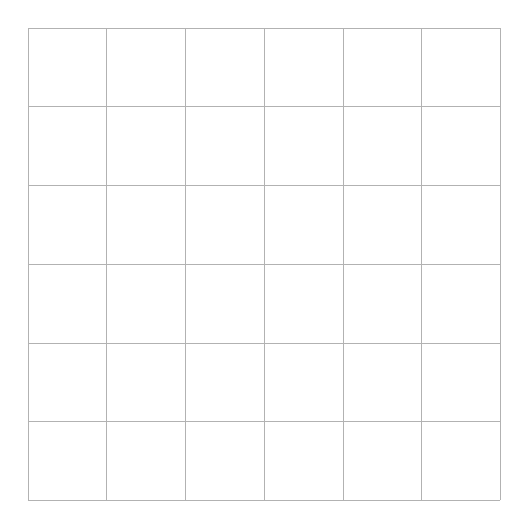
\begin{tikzpicture}
\draw (0,5) node {};
\draw (2,5) node {};
\draw (3,5) node {};
\draw[shift={(-0.5,-0.5)},black!30,very thin](0,0) grid (6,6);
\end{tikzpicture}
\quad
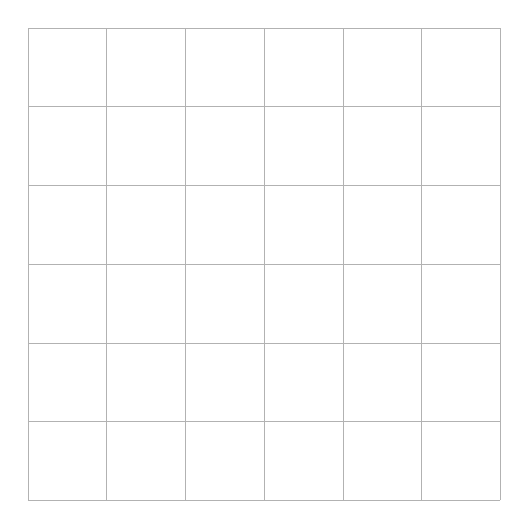
\begin{tikzpicture}
\draw (0,5) node {};
\draw (4,5) node {};
\draw (2,5) node {};
\draw (1,5) node {};
\draw (3,5) node {};
\draw (5,5) node {};
\draw[shift={(-0.5,-0.5)},black!30,very thin](0,0) grid (6,6);
\end{tikzpicture}
\quad
\left(\begin{array}{rrrr}
1&.&.&.\\
.&.&.&.\\
.&.&.&.\\
.&.&.&.\\
\end{array}\right)
\quad
\left(\begin{array}{rrrr}
1&1&.&.\\
.&.&.&.\\
.&.&.&.\\
.&.&.&.\\
\end{array}\right)
\quad
\left(\begin{array}{rrrr}
1&.&1&.\\
.&.&.&.\\
.&.&.&.\\
.&.&.&.
\\
\end{array}\right)
\quad
\left(\begin{array}{rrrr}
1&1&1&1\\
.&.&.&.\\
.&.&.&.\\
.&.&.&.\\
\end{array}\right)
\\
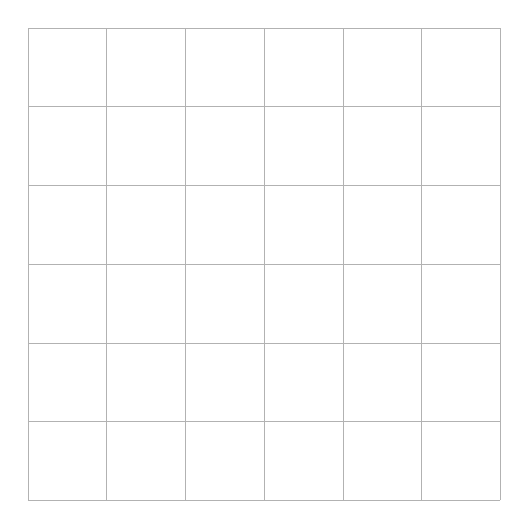
\begin{tikzpicture}
\draw (0,5) node {};
\draw (0,4) node {};
\draw[shift={(-0.5,-0.5)},black!30,very thin](0,0) grid (6,6);
\end{tikzpicture}
\quad
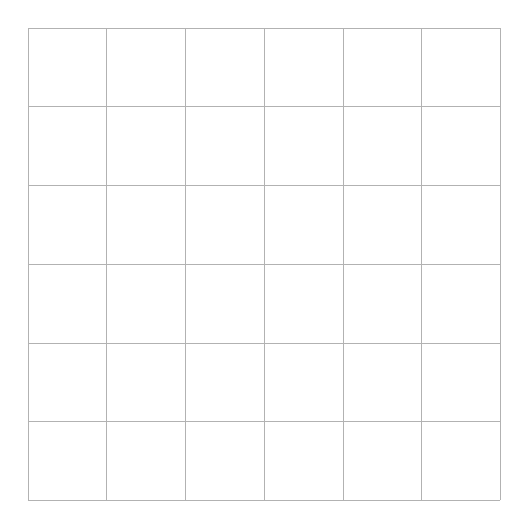
\begin{tikzpicture}
\draw (0,5) node {};
\draw (1,5) node {};
\draw (0,4) node {};
\draw (1,4) node {};
\draw[shift={(-0.5,-0.5)},black!30,very thin](0,0) grid (6,6);
\end{tikzpicture}
\quad
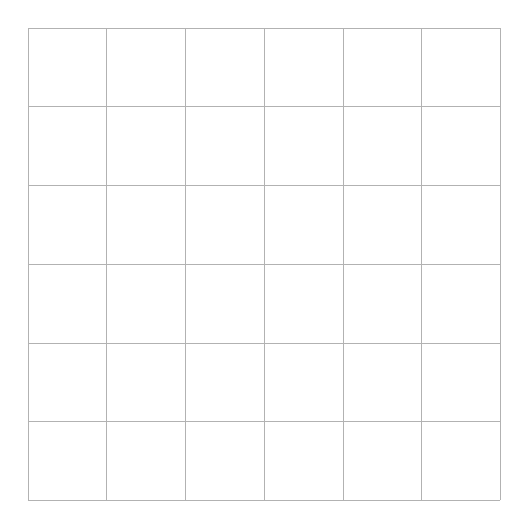
\begin{tikzpicture}
\draw (0,5) node {};
\draw (2,5) node {};
\draw (3,5) node {};
\draw (0,4) node {};
\draw (2,4) node {};
\draw (3,4) node {};
\draw[shift={(-0.5,-0.5)},black!30,very thin](0,0) grid (6,6);
\end{tikzpicture}
\quad
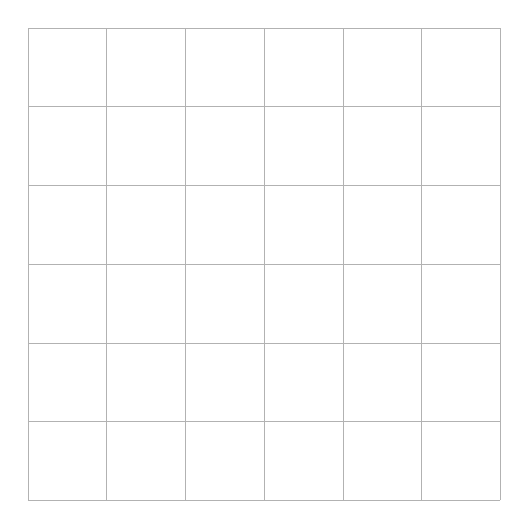
\begin{tikzpicture}
\draw (0,5) node {};
\draw (4,5) node {};
\draw (2,5) node {};
\draw (1,5) node {};
\draw (3,5) node {};
\draw (5,5) node {};
\draw (0,4) node {};
\draw (4,4) node {};
\draw (2,4) node {};
\draw (1,4) node {};
\draw (3,4) node {};
\draw (5,4) node {};
\draw[shift={(-0.5,-0.5)},black!30,very thin](0,0) grid (6,6);
\end{tikzpicture}
\quad
\left(\begin{array}{rrrr}
1&.&.&.\\
1&.&.&.\\
.&.&.&.\\
.&.&.&.\\
\end{array}\right)
\quad
\left(\begin{array}{rrrr}
1&1&.&.\\
1&1&.&.\\
.&.&.&.\\
.&.&.&.\\
\end{array}\right)
\quad
\left(\begin{array}{rrrr}
1&.&1&.\\
1&.&1&.\\
.&.&.&.\\
.&.&.&.\\
\end{array}\right)
\quad
\left(\begin{array}{rrrr}
1&1&1&1\\
1&1&1&1\\
.&.&.&.\\
.&.&.&.\\
\end{array}\right)
\\
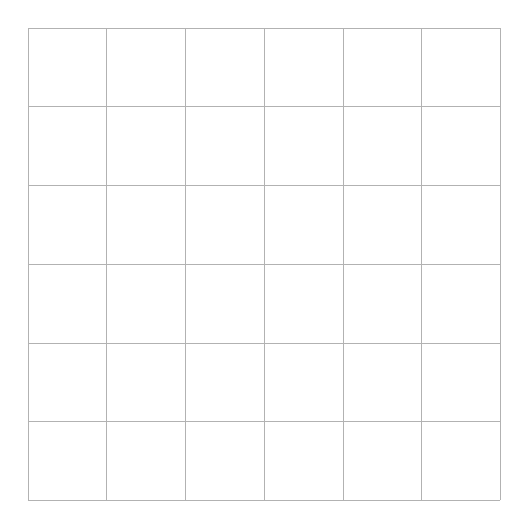
\begin{tikzpicture}
\draw (0,5) node {};
\draw (0,3) node {};
\draw (0,2) node {};
\draw[shift={(-0.5,-0.5)},black!30,very thin](0,0) grid (6,6);
\end{tikzpicture}
\quad
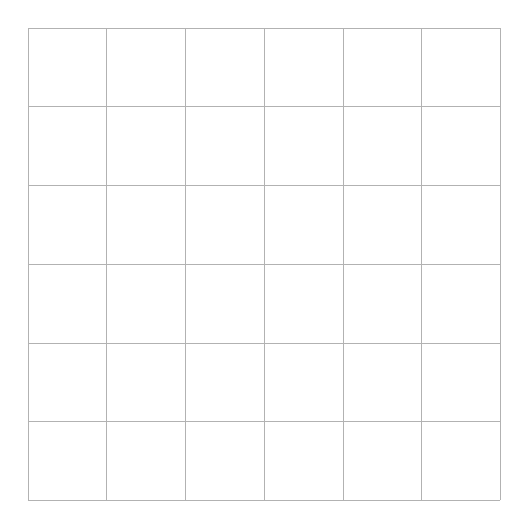
\begin{tikzpicture}
\draw (0,5) node {};
\draw (1,5) node {};
\draw (0,3) node {};
\draw (1,3) node {};
\draw (0,2) node {};
\draw (1,2) node {};
\draw[shift={(-0.5,-0.5)},black!30,very thin](0,0) grid (6,6);
\end{tikzpicture}
\quad
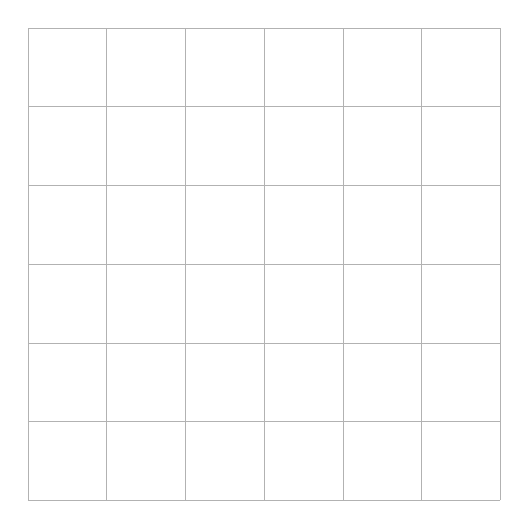
\begin{tikzpicture}
\draw (0,5) node {};
\draw (2,5) node {};
\draw (3,5) node {};
\draw (0,3) node {};
\draw (2,3) node {};
\draw (3,3) node {};
\draw (0,2) node {};
\draw (2,2) node {};
\draw (3,2) node {};
\draw[shift={(-0.5,-0.5)},black!30,very thin](0,0) grid (6,6);
\end{tikzpicture}
\quad
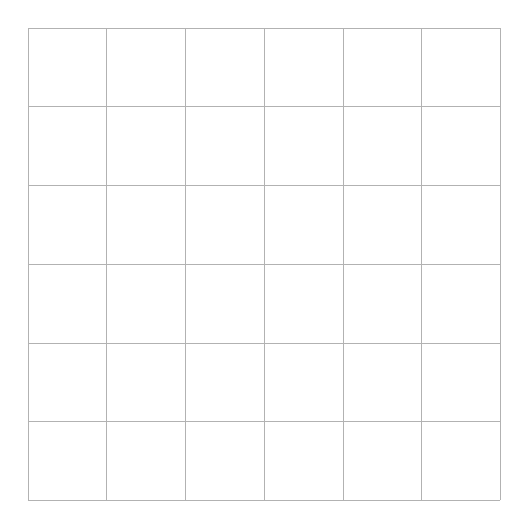
\begin{tikzpicture}
\draw (0,5) node {};
\draw (4,5) node {};
\draw (2,5) node {};
\draw (1,5) node {};
\draw (3,5) node {};
\draw (5,5) node {};
\draw (0,3) node {};
\draw (4,3) node {};
\draw (2,3) node {};
\draw (1,3) node {};
\draw (3,3) node {};
\draw (5,3) node {};
\draw (0,2) node {};
\draw (4,2) node {};
\draw (2,2) node {};
\draw (1,2) node {};
\draw (3,2) node {};
\draw (5,2) node {};
\draw[shift={(-0.5,-0.5)},black!30,very thin](0,0) grid (6,6);
\end{tikzpicture}
\quad
\left(\begin{array}{rrrr}
1&.&.&.\\
.&.&.&.\\
2&.&.&.\\
.&.&.&.\\
\end{array}\right)
\quad
\left(\begin{array}{rrrr}
1&1&.&.\\
.&.&.&.\\
2&2&.&.\\
.&.&.&.\\
\end{array}\right)
\quad
\left(\begin{array}{rrrr}
1&.&1&.\\
.&.&.&.\\
2&.&2&.\\
.&.&.&.\\
\end{array}\right)
\quad
\left(\begin{array}{rrrr}
1&1&1&1\\
.&.&.&.\\
2&2&2&2\\
.&.&.&.\\
\end{array}\right)
\\
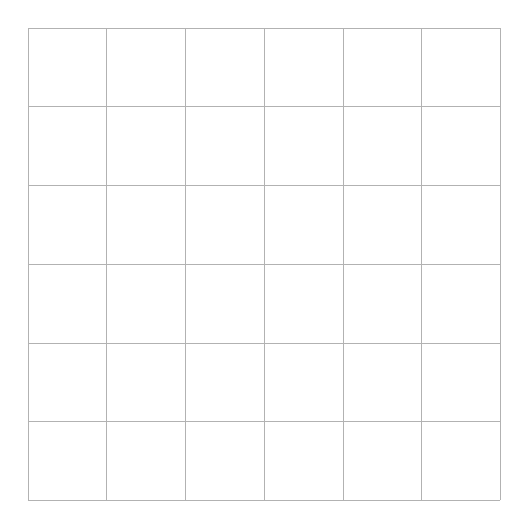
\begin{tikzpicture}
\draw (0,5) node {};
\draw (0,1) node {};
\draw (0,3) node {};
\draw (0,4) node {};
\draw (0,2) node {};
\draw (0,0) node {};
\draw[shift={(-0.5,-0.5)},black!30,very thin](0,0) grid (6,6);
\end{tikzpicture}
\quad
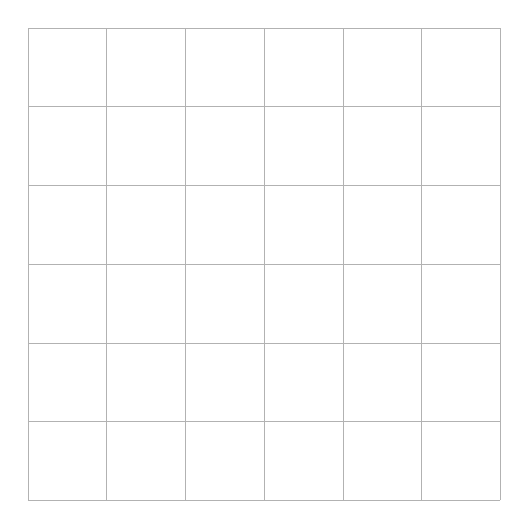
\begin{tikzpicture}
\draw (0,5) node {};
\draw (1,5) node {};
\draw (0,1) node {};
\draw (1,1) node {};
\draw (0,3) node {};
\draw (1,3) node {};
\draw (0,4) node {};
\draw (1,4) node {};
\draw (0,2) node {};
\draw (1,2) node {};
\draw (0,0) node {};
\draw (1,0) node {};
\draw[shift={(-0.5,-0.5)},black!30,very thin](0,0) grid (6,6);
\end{tikzpicture}
\quad
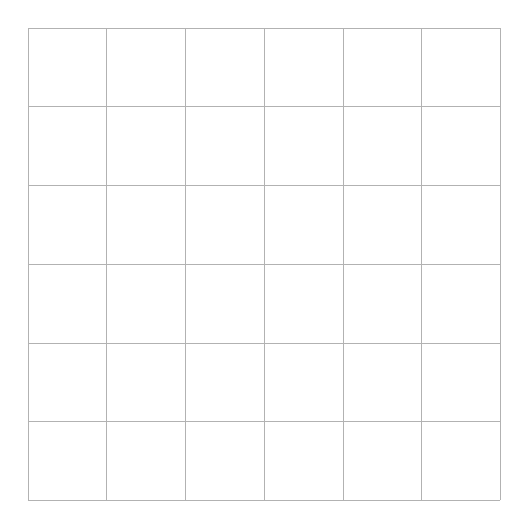
\begin{tikzpicture}
\draw (0,5) node {};
\draw (2,5) node {};
\draw (3,5) node {};
\draw (0,1) node {};
\draw (2,1) node {};
\draw (3,1) node {};
\draw (0,3) node {};
\draw (2,3) node {};
\draw (3,3) node {};
\draw (0,4) node {};
\draw (2,4) node {};
\draw (3,4) node {};
\draw (0,2) node {};
\draw (2,2) node {};
\draw (3,2) node {};
\draw (0,0) node {};
\draw (2,0) node {};
\draw (3,0) node {};
\draw[shift={(-0.5,-0.5)},black!30,very thin](0,0) grid (6,6);
\end{tikzpicture}
\quad
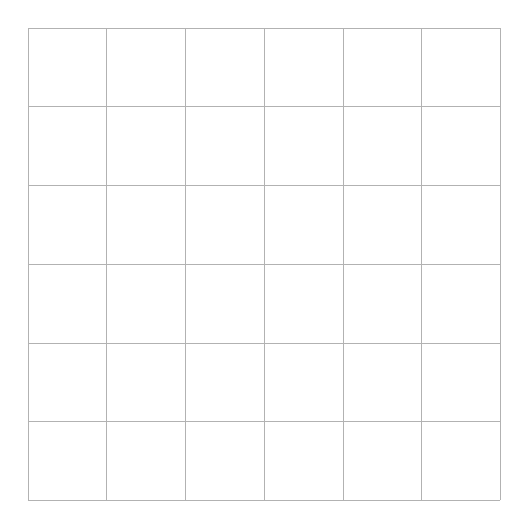
\begin{tikzpicture}
\draw (0,5) node {};
\draw (4,5) node {};
\draw (2,5) node {};
\draw (1,5) node {};
\draw (3,5) node {};
\draw (5,5) node {};
\draw (0,1) node {};
\draw (4,1) node {};
\draw (2,1) node {};
\draw (1,1) node {};
\draw (3,1) node {};
\draw (5,1) node {};
\draw (0,3) node {};
\draw (4,3) node {};
\draw (2,3) node {};
\draw (1,3) node {};
\draw (3,3) node {};
\draw (5,3) node {};
\draw (0,4) node {};
\draw (4,4) node {};
\draw (2,4) node {};
\draw (1,4) node {};
\draw (3,4) node {};
\draw (5,4) node {};
\draw (0,2) node {};
\draw (4,2) node {};
\draw (2,2) node {};
\draw (1,2) node {};
\draw (3,2) node {};
\draw (5,2) node {};
\draw (0,0) node {};
\draw (4,0) node {};
\draw (2,0) node {};
\draw (1,0) node {};
\draw (3,0) node {};
\draw (5,0) node {};
\draw[shift={(-0.5,-0.5)},black!30,very thin](0,0) grid (6,6);
\end{tikzpicture}
\quad
\left(\begin{array}{rrrr}
1&.&.&.\\
1&.&.&.\\
2&.&.&.\\
2&.&.&.\\
\end{array}\right)
\quad
\left(\begin{array}{rrrr}
1&1&.&.\\
1&1&.&.\\
2&2&.&.\\
2&2&.&.\\
\end{array}\right)
\quad
\left(\begin{array}{rrrr}
1&.&1&.\\
1&.&1&.\\
2&.&2&.\\
2&.&2&.\\
\end{array}\right)
\quad
\left(\begin{array}{rrrr}
1&1&1&1\\
1&1&1&1\\
2&2&2&2\\
2&2&2&2\\
\end{array}\right)
\\
\left(\begin{array}{rrrr|rr}
1&.&.&.&.&.\\
.&1&.&.&.&.\\
.&.&.&.&.&.\\
.&.&.&.&.&.\\ \hline
.&.&.&.&1&.\\
.&.&.&.&.&.\\
\end{array}\right)
\quad
\left(\begin{array}{rrrr|rr}
1&.&1&.&.&.\\
.&1&.&1&.&.\\
.&.&.&.&.&.\\
.&.&.&.&.&.\\ \hline
.&.&.&.&1&1\\
.&.&.&.&.&.\\
\end{array}\right)
\quad
\left(\begin{array}{rrrr|rr}
1&.&.&.&.&.\\
.&1&.&.&.&.\\
2&.&.&.&.&.\\
.&2&.&.&.&.\\ \hline
.&.&.&.&1&.\\
.&.&.&.&2&.\\
\end{array}\right)
\quad
\left(\begin{array}{rrrr|rr}
1&.&1&.&.&.\\
.&1&.&1&.&.\\
2&.&2&.&.&.\\
.&2&.&2&.&.\\ \hline
.&.&.&.&1&1\\
.&.&.&.&2&2\\
\end{array}\right)
\\
\left(\begin{array}{rrrr|rr|rrrr}
1&.&.&.&.&.&.&.&.&.\\
.&.&.&.&.&.&.&.&.&.\\
.&.&1&.&.&.&.&.&.&.\\
.&.&.&.&.&.&.&.&.&.\\ \hline
.&.&.&.&.&.&.&.&.&.\\
.&.&.&.&.&.&.&.&.&.\\ \hline
.&.&.&.&.&.&1&.&.&.\\
.&.&.&.&.&.&.&1&.&.\\
.&.&.&.&.&.&.&.&.&.\\
.&.&.&.&.&.&.&.&.&.\\
\end{array}\right)
\quad
\left(\begin{array}{rrrr|rr|rrrr}
1&.&.&.&.&.&.&.&.&.\\
.&.&.&.&.&.&.&.&.&.\\
.&.&1&.&.&.&.&.&.&.\\
.&.&.&.&.&.&.&.&.&.\\ \hline
.&.&.&.&.&.&.&.&.&.\\
.&.&.&.&.&.&.&.&.&.\\ \hline
.&.&.&.&.&.&.&1&.&.\\
.&.&.&.&.&.&1&.&.&.\\
.&.&.&.&.&.&.&.&.&.\\
.&.&.&.&.&.&.&.&.&.\\
\end{array}\right)
\quad
\left(\begin{array}{rrrr|rr|rrrr}
1&1&.&.&.&.&.&.&.&.\\
.&.&.&.&.&.&.&.&.&.\\
.&.&1&1&.&.&.&.&.&.\\
.&.&.&.&.&.&.&.&.&.\\ \hline
.&.&.&.&.&.&.&.&.&.\\
.&.&.&.&.&.&.&.&.&.\\ \hline
.&.&.&.&.&.&1&.&1&.\\
.&.&.&.&.&.&.&1&.&1\\
.&.&.&.&.&.&.&.&.&.\\
.&.&.&.&.&.&.&.&.&.\\
\end{array}\right)
\quad
\left(\begin{array}{rrrr|rr|rrrr}
1&1&.&.&.&.&.&.&.&.\\
.&.&.&.&.&.&.&.&.&.\\
.&.&1&1&.&.&.&.&.&.\\
.&.&.&.&.&.&.&.&.&.\\ \hline
.&.&.&.&.&.&.&.&.&.\\
.&.&.&.&.&.&.&.&.&.\\ \hline
.&.&.&.&.&.&.&1&.&1\\
.&.&.&.&.&.&1&.&1&.\\
.&.&.&.&.&.&.&.&.&.\\
.&.&.&.&.&.&.&.&.&.\\
\end{array}\right)
\\
\left(\begin{array}{rrrr|rr|rrrr}
1&.&.&.&.&.&.&.&.&.\\
1&.&.&.&.&.&.&.&.&.\\
.&.&1&.&.&.&.&.&.&.\\
.&.&1&.&.&.&.&.&.&.\\ \hline
.&.&.&.&.&.&.&.&.&.\\
.&.&.&.&.&.&.&.&.&.\\ \hline
.&.&.&.&.&.&1&.&.&.\\
.&.&.&.&.&.&.&1&.&.\\
.&.&.&.&.&.&1&.&.&.\\
.&.&.&.&.&.&.&1&.&.\\
\end{array}\right)
\quad
\left(\begin{array}{rrrr|rr|rrrr}
1&.&.&.&.&.&.&.&.&.\\
1&.&.&.&.&.&.&.&.&.\\
.&.&1&.&.&.&.&.&.&.\\
.&.&1&.&.&.&.&.&.&.\\ \hline
.&.&.&.&.&.&.&.&.&.\\
.&.&.&.&.&.&.&.&.&.\\ \hline
.&.&.&.&.&.&.&1&.&.\\
.&.&.&.&.&.&1&.&.&.\\
.&.&.&.&.&.&.&1&.&.\\
.&.&.&.&.&.&1&.&.&.\\
\end{array}\right)
\quad
\left(\begin{array}{rrrr|rr|rrrr}
1&1&.&.&.&.&.&.&.&.\\
1&1&.&.&.&.&.&.&.&.\\
.&.&1&1&.&.&.&.&.&.\\
.&.&1&1&.&.&.&.&.&.\\ \hline
.&.&.&.&.&.&.&.&.&.\\
.&.&.&.&.&.&.&.&.&.\\ \hline
.&.&.&.&.&.&1&.&1&.\\
.&.&.&.&.&.&.&1&.&1\\
.&.&.&.&.&.&1&.&1&.\\
.&.&.&.&.&.&.&1&.&1\\
\end{array}\right)
\quad
\left(\begin{array}{rrrr|rr|rrrr}
1&1&.&.&.&.&.&.&.&.\\
1&1&.&.&.&.&.&.&.&.\\
.&.&1&1&.&.&.&.&.&.\\
.&.&1&1&.&.&.&.&.&.\\ \hline
.&.&.&.&.&.&.&.&.&.\\
.&.&.&.&.&.&.&.&.&.\\ \hline
.&.&.&.&.&.&.&1&.&1\\
.&.&.&.&.&.&1&.&1&.\\
.&.&.&.&.&.&.&1&.&1\\
.&.&.&.&.&.&1&.&1&.\\
\end{array}\right)
\\
\left(\begin{array}{rrrr|rr|rrrr|rr}
1&.&.&.&.&.&.&.&.&.&.&.\\
.&1&.&.&.&.&.&.&.&.&.&.\\
.&.&1&.&.&.&.&.&.&.&.&.\\
.&.&.&1&.&.&.&.&.&.&.&.\\ \hline
.&.&.&.&1&.&.&.&.&.&.&.\\
.&.&.&.&.&1&.&.&.&.&.&.\\ \hline
.&.&.&.&.&.&1&.&.&.&.&.\\
.&.&.&.&.&.&.&1&.&.&.&.\\
.&.&.&.&.&.&.&.&1&.&.&.\\
.&.&.&.&.&.&.&.&.&1&.&.\\ \hline
.&.&.&.&.&.&.&.&.&.&1&.\\
.&.&.&.&.&.&.&.&.&.&.&1\\
\end{array}\right)
\quad
\left(\begin{array}{rrrr|rr|rrrr|rr}
1&.&.&.&.&.&.&.&.&.&.&.\\
.&1&.&.&.&.&.&.&.&.&.&.\\
.&.&1&.&.&.&.&.&.&.&.&.\\
.&.&.&1&.&.&.&.&.&.&.&.\\ \hline
.&.&.&.&1&.&.&.&.&.&.&.\\
.&.&.&.&.&1&.&.&.&.&.&.\\ \hline
.&.&.&.&.&.&.&1&.&.&.&.\\
.&.&.&.&.&.&1&.&.&.&.&.\\
.&.&.&.&.&.&.&.&.&1&.&.\\
.&.&.&.&.&.&.&.&1&.&.&.\\ \hline
.&.&.&.&.&.&.&.&.&.&.&1\\
.&.&.&.&.&.&.&.&.&.&1&.\\
\end{array}\right)
\quad
% gap> LogTo();
\end{align*}

% gap> for r in reps do
% > Print(TikzRelationSubgroup(GG, elm, r));
% > Print("\\quad\n");
% > od;
\begin{center}
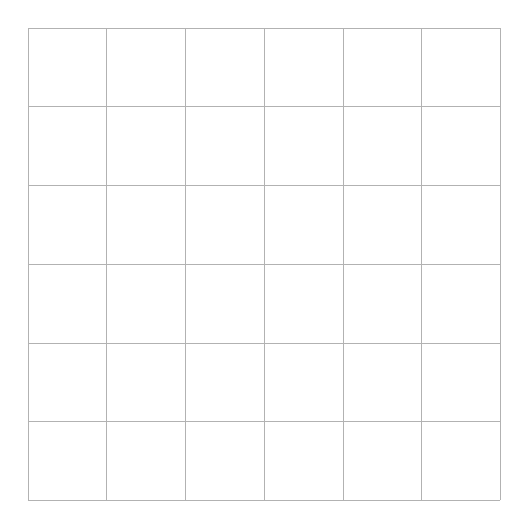
\begin{tikzpicture}
\draw (0,5) node {};
\draw (0,1) node {};
\draw (0,3) node {};
\draw (0,4) node {};
\draw (0,2) node {};
\draw (0,0) node {};
\draw[shift={(-0.5,-0.5)},black!30,very thin](0,0) grid (6,6);
\end{tikzpicture}
\quad
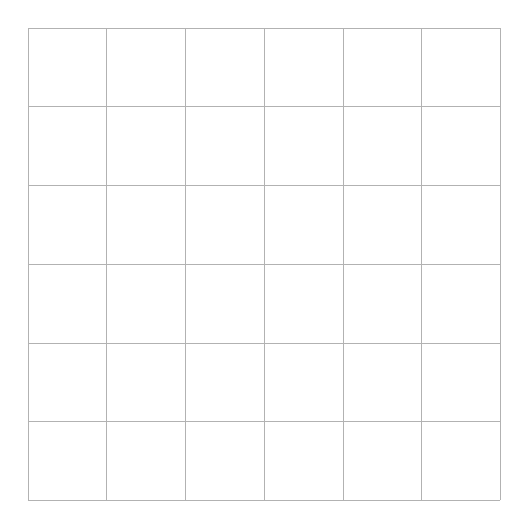
\begin{tikzpicture}
\draw (0,5) node {};
\draw (1,5) node {};
\draw (0,1) node {};
\draw (1,1) node {};
\draw (0,3) node {};
\draw (1,3) node {};
\draw (0,4) node {};
\draw (1,4) node {};
\draw (0,2) node {};
\draw (1,2) node {};
\draw (0,0) node {};
\draw (1,0) node {};
\draw[shift={(-0.5,-0.5)},black!30,very thin](0,0) grid (6,6);
\end{tikzpicture}
\quad
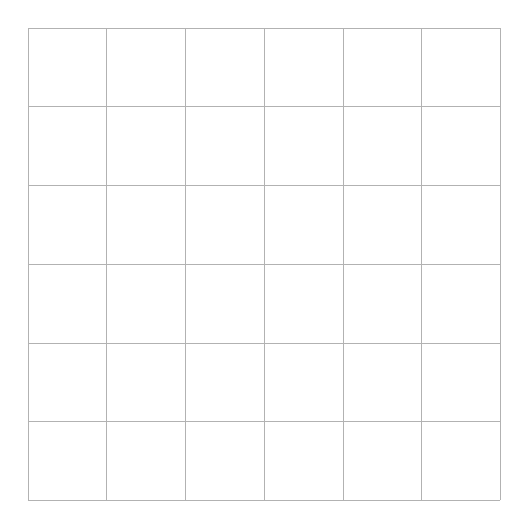
\begin{tikzpicture}
\draw (0,5) node {};
\draw (2,5) node {};
\draw (3,5) node {};
\draw (0,1) node {};
\draw (2,1) node {};
\draw (3,1) node {};
\draw (0,3) node {};
\draw (2,3) node {};
\draw (3,3) node {};
\draw (0,4) node {};
\draw (2,4) node {};
\draw (3,4) node {};
\draw (0,2) node {};
\draw (2,2) node {};
\draw (3,2) node {};
\draw (0,0) node {};
\draw (2,0) node {};
\draw (3,0) node {};
\draw[shift={(-0.5,-0.5)},black!30,very thin](0,0) grid (6,6);
\end{tikzpicture}
\quad
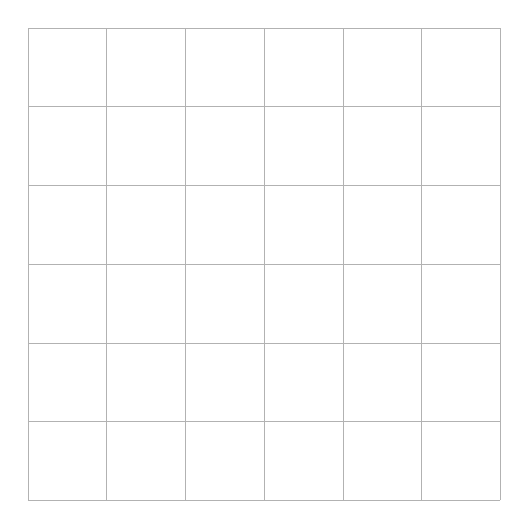
\begin{tikzpicture}
\draw (0,5) node {};
\draw (4,5) node {};
\draw (2,5) node {};
\draw (1,5) node {};
\draw (3,5) node {};
\draw (5,5) node {};
\draw (0,1) node {};
\draw (4,1) node {};
\draw (2,1) node {};
\draw (1,1) node {};
\draw (3,1) node {};
\draw (5,1) node {};
\draw (0,3) node {};
\draw (4,3) node {};
\draw (2,3) node {};
\draw (1,3) node {};
\draw (3,3) node {};
\draw (5,3) node {};
\draw (0,4) node {};
\draw (4,4) node {};
\draw (2,4) node {};
\draw (1,4) node {};
\draw (3,4) node {};
\draw (5,4) node {};
\draw (0,2) node {};
\draw (4,2) node {};
\draw (2,2) node {};
\draw (1,2) node {};
\draw (3,2) node {};
\draw (5,2) node {};
\draw (0,0) node {};
\draw (4,0) node {};
\draw (2,0) node {};
\draw (1,0) node {};
\draw (3,0) node {};
\draw (5,0) node {};
\draw[shift={(-0.5,-0.5)},black!30,very thin](0,0) grid (6,6);
\end{tikzpicture}
\quad
\begin{tikzpicture}
\draw (0,5) node {};
\draw (1,4) node {};
\draw[shift={(-0.5,-0.5)},black!30,very thin](0,0) grid (6,6);
\end{tikzpicture}
\quad
\begin{tikzpicture}
\draw (0,5) node {};
\draw (2,5) node {};
\draw (3,5) node {};
\draw (4,4) node {};
\draw (1,4) node {};
\draw (5,4) node {};
\draw[shift={(-0.5,-0.5)},black!30,very thin](0,0) grid (6,6);
\end{tikzpicture}
\quad
\begin{tikzpicture}
\draw (0,5) node {};
\draw (1,1) node {};
\draw (0,3) node {};
\draw (1,4) node {};
\draw (0,2) node {};
\draw (1,0) node {};
\draw[shift={(-0.5,-0.5)},black!30,very thin](0,0) grid (6,6);
\end{tikzpicture}
\quad
\begin{tikzpicture}
\draw (0,5) node {};
\draw (2,5) node {};
\draw (3,5) node {};
\draw (4,1) node {};
\draw (1,1) node {};
\draw (5,1) node {};
\draw (0,3) node {};
\draw (2,3) node {};
\draw (3,3) node {};
\draw (4,4) node {};
\draw (1,4) node {};
\draw (5,4) node {};
\draw (0,2) node {};
\draw (2,2) node {};
\draw (3,2) node {};
\draw (4,0) node {};
\draw (1,0) node {};
\draw (5,0) node {};
\draw[shift={(-0.5,-0.5)},black!30,very thin](0,0) grid (6,6);
\end{tikzpicture}
\quad
\begin{tikzpicture}
\draw (0,5) node {};
\draw (2,3) node {};
\draw (3,2) node {};
\draw[shift={(-0.5,-0.5)},black!30,very thin](0,0) grid (6,6);
\end{tikzpicture}
\quad
\begin{tikzpicture}
\draw (0,5) node {};
\draw (3,3) node {};
\draw (2,2) node {};
\draw[shift={(-0.5,-0.5)},black!30,very thin](0,0) grid (6,6);
\end{tikzpicture}
\quad
\begin{tikzpicture}
\draw (0,5) node {};
\draw (1,5) node {};
\draw (2,3) node {};
\draw (5,3) node {};
\draw (4,2) node {};
\draw (3,2) node {};
\draw[shift={(-0.5,-0.5)},black!30,very thin](0,0) grid (6,6);
\end{tikzpicture}
\quad
\begin{tikzpicture}
\draw (0,5) node {};
\draw (1,5) node {};
\draw (4,3) node {};
\draw (3,3) node {};
\draw (2,2) node {};
\draw (5,2) node {};
\draw[shift={(-0.5,-0.5)},black!30,very thin](0,0) grid (6,6);
\end{tikzpicture}
\quad
\begin{tikzpicture}
\draw (0,5) node {};
\draw (3,1) node {};
\draw (2,3) node {};
\draw (0,4) node {};
\draw (3,2) node {};
\draw (2,0) node {};
\draw[shift={(-0.5,-0.5)},black!30,very thin](0,0) grid (6,6);
\end{tikzpicture}
\quad
\begin{tikzpicture}
\draw (0,5) node {};
\draw (2,1) node {};
\draw (3,3) node {};
\draw (0,4) node {};
\draw (2,2) node {};
\draw (3,0) node {};
\draw[shift={(-0.5,-0.5)},black!30,very thin](0,0) grid (6,6);
\end{tikzpicture}
\quad
\begin{tikzpicture}
\draw (0,5) node {};
\draw (1,5) node {};
\draw (4,1) node {};
\draw (3,1) node {};
\draw (2,3) node {};
\draw (5,3) node {};
\draw (0,4) node {};
\draw (1,4) node {};
\draw (4,2) node {};
\draw (3,2) node {};
\draw (2,0) node {};
\draw (5,0) node {};
\draw[shift={(-0.5,-0.5)},black!30,very thin](0,0) grid (6,6);
\end{tikzpicture}
\quad
\begin{tikzpicture}
\draw (0,5) node {};
\draw (1,5) node {};
\draw (2,1) node {};
\draw (5,1) node {};
\draw (4,3) node {};
\draw (3,3) node {};
\draw (0,4) node {};
\draw (1,4) node {};
\draw (2,2) node {};
\draw (5,2) node {};
\draw (4,0) node {};
\draw (3,0) node {};
\draw[shift={(-0.5,-0.5)},black!30,very thin](0,0) grid (6,6);
\end{tikzpicture}
\quad
\begin{tikzpicture}
\draw (0,5) node {};
\draw (4,1) node {};
\draw (2,3) node {};
\draw (1,4) node {};
\draw (3,2) node {};
\draw (5,0) node {};
\draw[shift={(-0.5,-0.5)},black!30,very thin](0,0) grid (6,6);
\end{tikzpicture}
\quad
\begin{tikzpicture}
\draw (0,5) node {};
\draw (5,1) node {};
\draw (3,3) node {};
\draw (1,4) node {};
\draw (2,2) node {};
\draw (4,0) node {};
\draw[shift={(-0.5,-0.5)},black!30,very thin](0,0) grid (6,6);
\end{tikzpicture}
\end{center}
% gap> LogTo();
\end{document}
